\documentclass[12pt,a4paper]{report}
%\usepackage[fontsize=14pt]{scrextend}
\setcounter{secnumdepth}{3}
\usepackage[a4paper, bindingoffset=0cm,
            left=2.5cm, right=3cm, top=2.5cm, bottom=2.5cm,
            footskip=1cm]{geometry}
\usepackage{hyperref}
\hypersetup{
    colorlinks=true,
    citecolor=blue,
    filecolor=blue,
    linkcolor=blue,
    urlcolor=blue
}
\usepackage{floatrow}
\DeclareFloatFont{foot}{\footnotesize}% "scriptsize" is defined by floatrow, "tiny" not
\floatsetup[table]{font=foot}
\usepackage{titlesec}
\usepackage{setspace}
\usepackage{graphicx}
\usepackage{subfig}
\usepackage[font={small},labelfont={small}]{caption}
\usepackage{float}
\floatstyle{plaintop}
\restylefloat{table}
\usepackage[extrafootnotefeatures]{xepersian}
\newcommand{\HRule}{\rule{\linewidth}{2.5mm}}
\settextfont[Scale=1]{IRXLotus}
\setlatintextfont[Scale=0.82]{Times New Roman}
\setdigitfont{IRXLotus}

% ---------------------------------------------------------------------- Commands
\makeatletter
\newcommand\thefontsize[1]{{#1 The current font size is: \f@size pt\par}}
\makeatother

\makeatletter %only needed in preamble
\renewcommand\footnotesize{\@setfontsize\footnotesize{10pt}{12}}   % Footnote/Table 10pt
\renewcommand\small{\@setfontsize\small{12pt}{14.4}} % Caption/Abstract/References 12pt
\renewcommand\normalsize{\@setfontsize\normalsize{14pt}{16.8}} % Titre far-e 14pt
\renewcommand\large{\@setfontsize\large{16pt}{19.2}} % Titre asli/Section 16pt
\renewcommand\Large{\@setfontsize\Large{18pt}{21.6}} % Onvane fasl/Chapter 18pt
\makeatother
% -------------------------------------------------------------------------------

% ------------------------------------------------------------------ Title Format
%\titleformat{\chapter}[display]
%  {\Large\bfseries}{\filcenter\chaptertitlename\ \thechapter}
\titleformat{\chapter}{\Large\bfseries\Large}{فصل \thechapter}{18pt}{}
\titleformat*{\section}{\large\bfseries}
\titleformat*{\subsection}{\normalsize\bfseries}
\titleformat*{\subsubsection}{\normalsize\bfseries}
\titleformat*{\paragraph}{\normalsize\bfseries}
\titleformat*{\subparagraph}{\normalsize\bfseries}
% --------------------------------------------------------------------------------


\begin{document}
\begin{titlepage}
	\begin{center}
		$ $\\[2cm]
		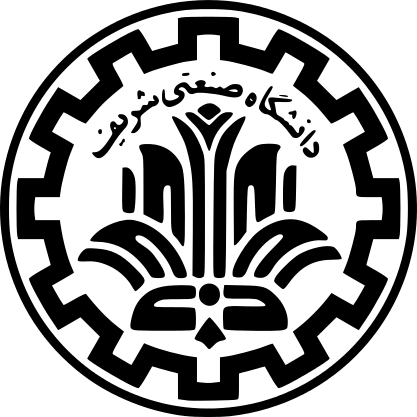
\includegraphics[width=3cm]{Images//Shariflogo.png}\\
        \textbf{\Large دانشگاه صنعتی شریف}\\
		\textsc{\Large دانشکده مهندسی برق}\\[2cm]
		\textbf{\Large ‌‌گزارش پروژه یادگیری عمیق}\\[2cm]
		\textbf{\large نگارش}\\[0.3cm]
		\textsc{\large پوریا اشرفیان (96101227)}\\[0.3cm]
		\textsc{\large میلاد صمیمی‌فر (400205577)}\\[0.6cm]
		\textsc{\large بهمن 1400}\\[1cm]
	\end{center}
\end{titlepage}
\thispagestyle{empty}
‎\renewcommand{\baselinestretch}{1.5}\normalsize‎
\renewcommand{\bibname}{مراجع}
\renewcommand{\listfigurename}{فهرست شکل‌ها}
\renewcommand{\listtablename}{فهرست جدول‌ها}

\pagenumbering{alph}
\setcounter{page}{2}
\tableofcontents
\addtocontents{toc}{\textbf{فهرست مطالب}~\hfill\textbf{\thepage}\par}

%\listoftables
%\addtocontents{toc}{\textbf{فهرست جدول‌ها}~\hfill\textbf{\thepage}\par}
%
%\listoffigures
%\addtocontents{toc}{\textbf{فهرست شکل‌ها}~\hfill\textbf{\thepage}\par}

\chapter{تشخیص اشیاء} \pagenumbering{arabic}
در این قسمت از مدل آماده \lr{YOLO-v3} استفاده کردیم. این مدل با توجه به ساختاری که دارد در پردازش‌های \lr{real-time} استفاده می‌شود و سرعت بالایی در یافتن اشیا دارد.
\begin{figure}[h]
  \centering
  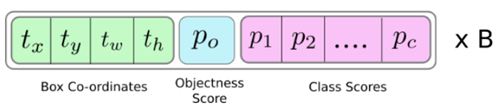
\includegraphics[width=0.5\textwidth]{Images//yolo1.png}
  \caption{خروجی‌های شبکه \lr{YOLO-v3}}
  \label{yolo1}
\end{figure}

همان طور که از تصویر \ref{yolo1} مشخص است خروجی این مدل حاوی مختصات bounding box های اشیای تشخیص داده شده‌است که در قسمت اتصال دو مدل تشخیص عمق و تشخیص اشیا از این خاصیت استفاده می‌کنیم.

در ادامه روش اصلی و مزیت‌های \lr{YOLO-v3} نسبت به ورژن‌های قبلی \lr{YOLO} را بیان می‌کنیم.
در این روش برای تشخیص صحیح‌تر داده هایی که دارای اشیا با پراکندگی اندازه‌های بالا\LTRfootnote{High Size Variation} هستند، چند روش استفاده شده که یکی از این روش‌ها \lr{Predictions Across Scales} نام دارد. برای این کار از مفهوم \lr{Feature Pyramid Networks} بهره گرفته شده‌است. در این شبکه برای هر \lr{scale} سه باکس پیش‌بینی می شود.

در مرحله بعد \lr{feature map} دو لایه پیشین را با ضریب ۲ \lr{upsample} کرده و با \lr{feature map} خود ترکیب می‌کنیم (concatenate). با همین روش \lr{scale} سوم را هم میسازیم. با توجه به این که در مرحله آخر از مراحل قبلی استفاده میکنیم، از محاسبات قبلی به نحو احسن استفاده می شود و مشکل پراکندگی اندازه های بالا کمتر پیش خواهد آمد.
در شکل‌های \ref{yolo2} و \ref{yolo3} به ترتیب نمای کلی و ساختار شبکه \lr{YOLO-v3} آمده است.

معیار ارزیابی مدلی که ما استفاده کردیم
\lr{mAP}\LTRfootnote{Mean Average Precision}
است و مقدار آن برای این مدل $57.9$ درصد است.
این مدل از
\href{https://pjreddie.com/darknet/yolo}{pjreddie.com/darknet/yolo}
قابل دانلود است.
\begin{figure}
  \centering
  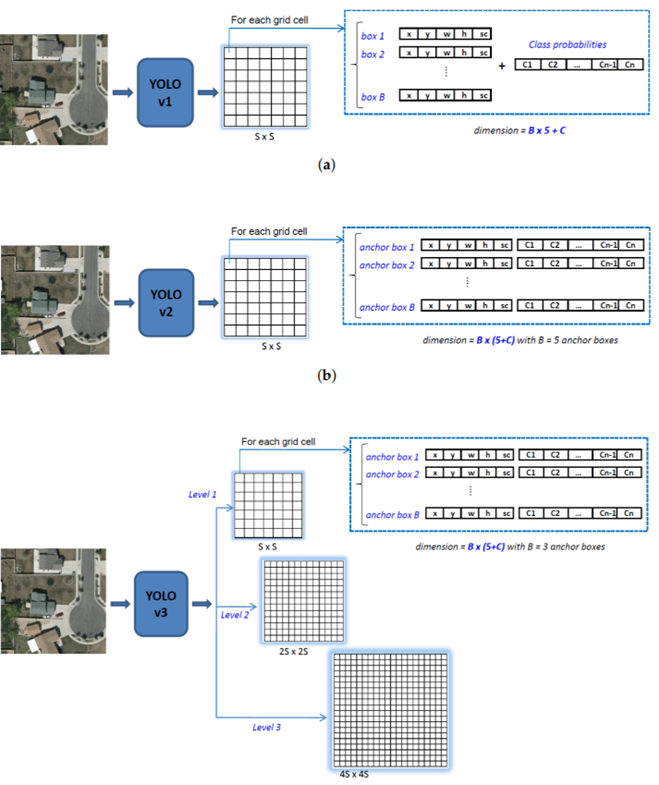
\includegraphics[width=\textwidth]{Images//yolo2.png}
  \caption{نمای کلی \lr{YOLO-v3}}\label{yolo2}
\end{figure}
\begin{figure}
  \centering
  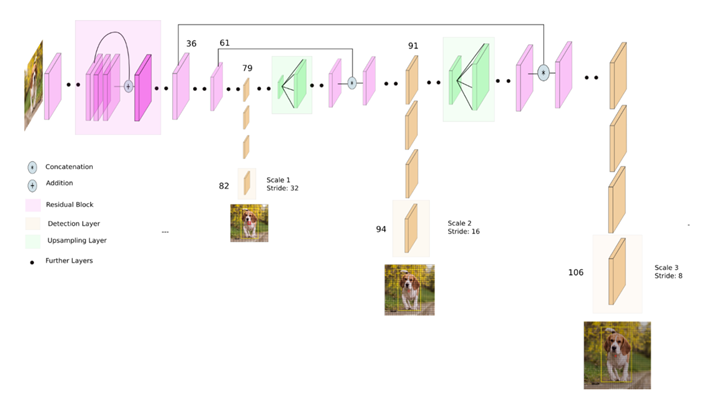
\includegraphics[width=\textwidth]{Images//yolo3.png}
  \caption{ساختار شبکه \lr{YOLO-v3}}\label{yolo3}
\end{figure}

در شکل \ref{yolo4} تابع هزینه شبکه \lr{YOLO-v2} آمده‌است.
در شبکه ما به جای مربعات از آنتروپی متقابل استفاده می‌شود.
بنابراین به نوعی در این ورژن از \lr{logistic regression} برای به محاسبه \lr{confidence} و \lr{predictions} استفاده می‌کنیم.
مفهوم کلی این تابع هزینه به این معنی است که برای هر \lr{ground truth box} باکس خود را تولید می‌کنیم به طوری که بیشترین همپوشانی را با باکس اصلی داشته باشد.
\begin{figure}
  \centering
  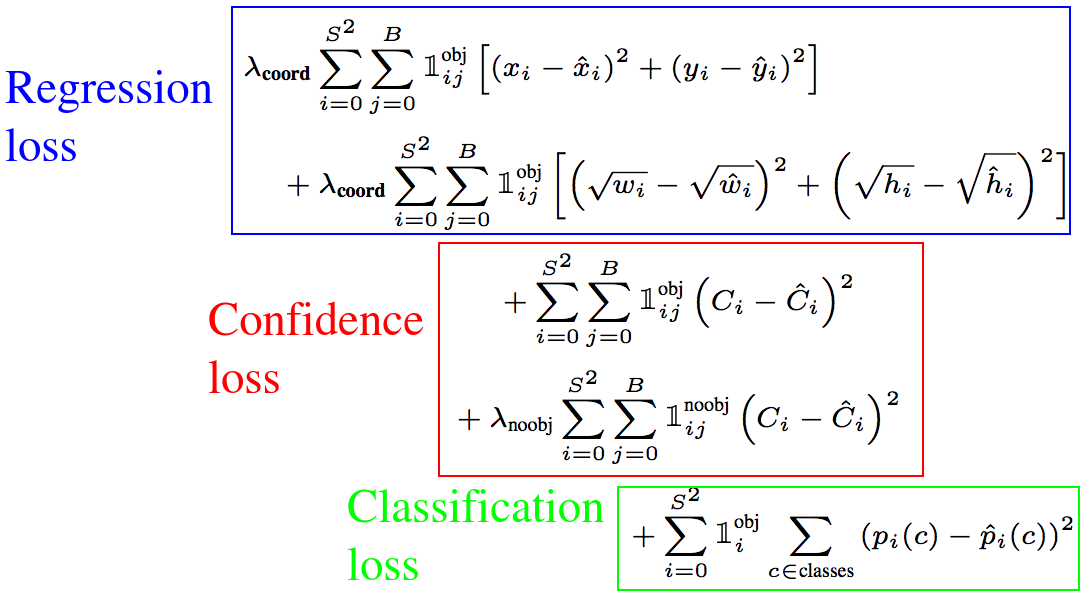
\includegraphics[width=.8\textwidth]{Images//yolo4.png}
  \caption{تابع هزینه \lr{YOLO-v2}}\label{yolo4}
\end{figure}


\chapter{تشخیص عمق}

\section{ساختار \lr{CycleGAN}}
این روش اولین بار در \cite{zhu2020unpaired} ارائه شد.
در این روش به دنبال یافتن دو تبدیل $G$ و $F$
هستیم که از دامنه تصاویر \lr{RGB} به تصاویر عمق
و برعکس کار می‌کنند. همچنین به دنبال این هستیم که این دو تبدیل معکوس یکدیگر باشند.
تابع هزینه مورد استفاده در این روش در شکل \ref{cg_loss} آمده‌است.
علاوه بر شبکه‌های $G$ و $F$،
دو شبکه تمایزدهنده برای $D_X$ و $D_Y$
برای دامنه‌های تصاویر اصلی و تصاویر عمق وجود دارند که برخلاف شبکه های مولد عمل می‌کنند.
ترم اول و دوم مربوط به این شبکه‌هاست و به صورت میانگین مربعات تفاضل پیکسل‌های لابه
آخر با ماتریس یکانی محاسبه می‌شوند.
ترم سوم برای اجبار به معکوس بودن تبدیل‌های مولد است و در شکل \ref{cg_cycle} آمده‌است.
\begin{figure}[h]
  \centering
  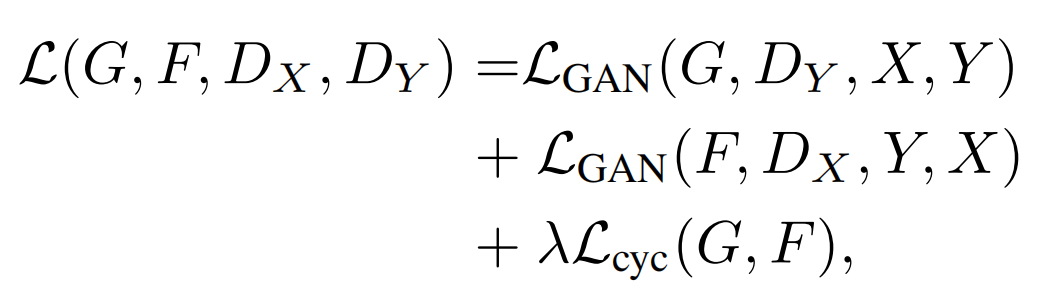
\includegraphics[width=.5\textwidth]{Images//cg1.png}
  \caption{تابع هزینه مورد استفاده در \lr{CycleGAN}}\label{cg_loss}
\end{figure}
\begin{figure}[h]
  \centering
  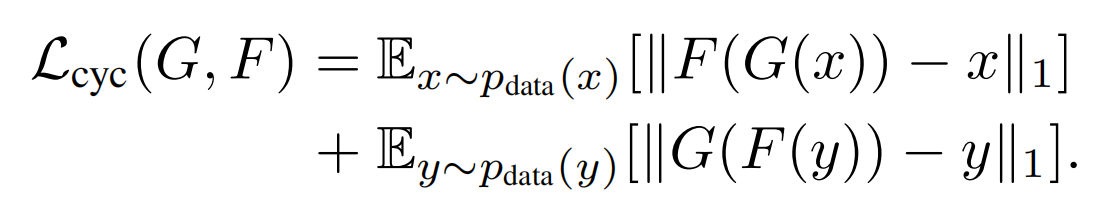
\includegraphics[width=.5\textwidth]{Images//cg2.png}
  \caption{ترم هزینه مربوط به معکوس بودن}\label{cg_cycle}
\end{figure}

شبکه‌های $G$ و $F$ هر کدام شامل
2 بلوک \lr{downsampling}، پنج \lr{resblock} و دو بلوک \lr{upsampling}
هستند. شبکه های $D$ هم شامل سه بلوک \lr{downsampling} هستند.
جزئیات لایه‌های این شبکه‌ها در نوت بوک مربوطه وجود دارد.
بهترین شبیه‌سازی انجام شده
روی این مدل با بهینه‌ساز آدام، نرخ یادگیری $0.0002$
و مقدار $\beta_1$ برابر با $0.5$ انجام شد.
معیار ارزیابی \lr{RMS}\LTRfootnote{Root Mean Squared}
بود که پس از 20 مرحله آموزش با سایز بچ 1 به $0.3$
روی داده‌های تست رسید.
در طول آموزش 1100 تصویر برای آموزش و 349 تصویر برای تست استفاده شدند.
در شکل \ref{cg_test} نتیجه تست شبکه روی تعدادی از داده های تست آورده شده‌است.
چون با شبیه سازی های متوالی نتایج به حد مطلوبمان نرسید به سراغ شبکه \lr{Unet} رفتیم.
\begin{figure}
  \centering
  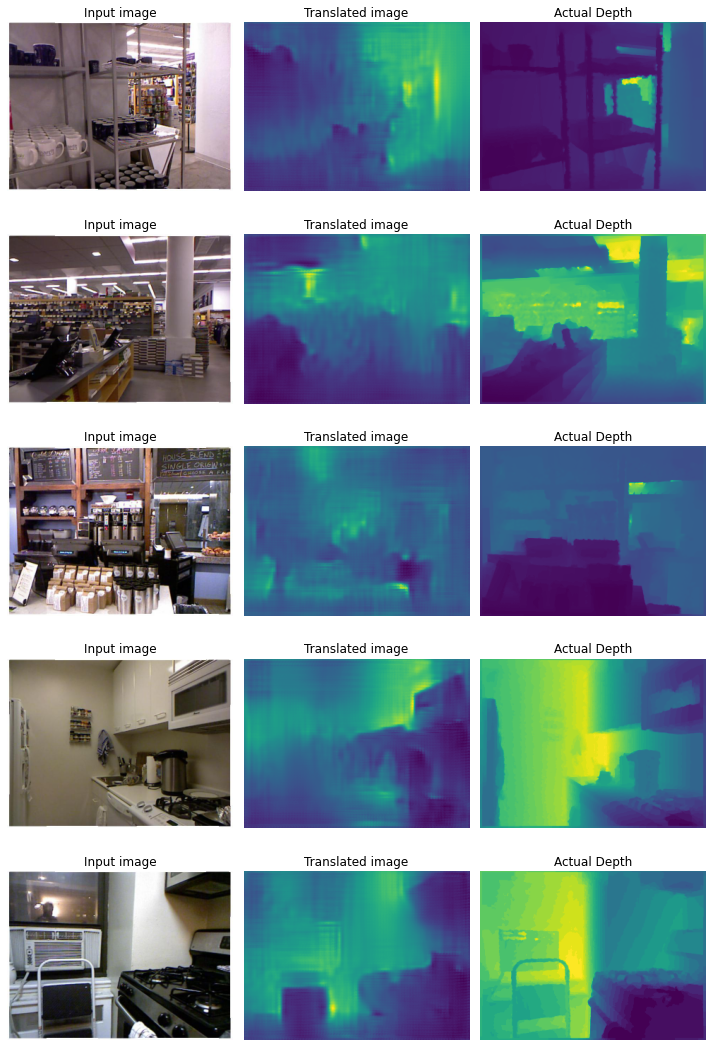
\includegraphics[width=.5\textwidth]{Images//cg3.png}
  \caption{نتایح تست شبکه \lr{CycleGAN} آموزش دیده}\label{cg_test}
\end{figure}

\section{ساختار \lr{Unet}}
این ساختار را از \cite{alhashim2019high} برداشتیم.
همان طور از در شکل \ref{unet_str} دیده می‌شود، شبکه شامل یک انکودر و دکودر است.
انکودر شبکه شامل یک تقطیع از شبکه \lr{DenseNet-169} است.
انکودر ورودی را به یک بردار ویژگی تبدیل می‌کند،
سپس دکودر با \lr{upsample}های متوالی آن را به تصویر
عمق خروجی تبدیل می‌کند. جزئیات لایه‌ها در جدول \ref{unet_table}
و در نوت‌بوک مربوطه وجود دارند.
\begin{figure}
  \centering
  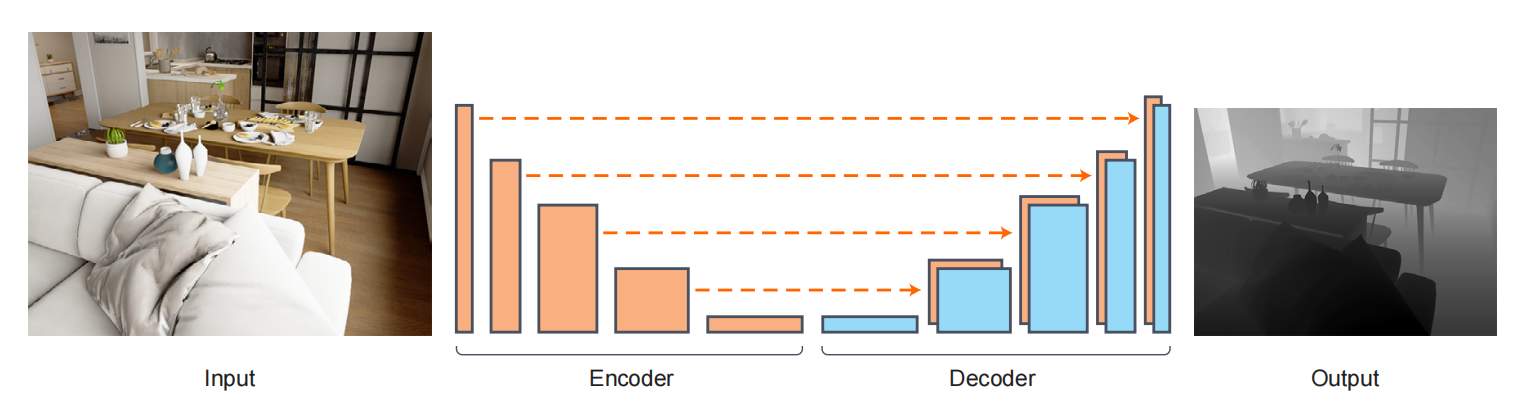
\includegraphics[width=.8\textwidth]{Images//unet1.png}
  \caption{نمای کلی شبکه}\label{unet_str}
\end{figure}
\begin{table}
  \centering
  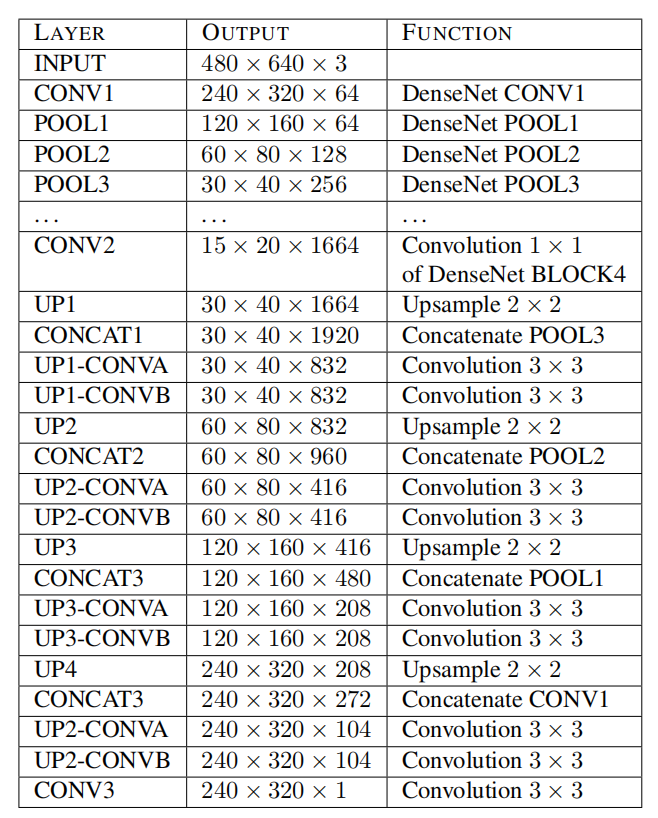
\includegraphics[width=.5\textwidth]{Images//unet8.png}
  \caption{لایه های شبکه؛ تا قبل از لایه \lr{UP1} تمام لایه ها، لایه های \lr{DenseNet-169} هستند.}\label{unet_table}
\end{table}

80 درصد داده‌ها برای آموزش استفاده شدند،
10 دصد برای اعتبارسنجی و 10 درصد برای تست.
معیار ارزیابی روش ما با مقاله فرق دارد.
صحت ما به این صورت تعریف می شود که خروجی پیکسل‌های خروجی شبکه
(که خروجی یک تابع سیگوید هستند)
به نزدیک ترین عدد صحیح (0 تا 1)
گرد می‌شوند.
سپس همین اتفاق برای پیکسل‌های خروجی واقعی (که مقادیرشان بین صفر و 1 نرمالیزه شده‌اند)
انجام می‌شود.
مقادیر حاصل در پیکسل‌ها تک به تک مقایسه می‌شوند و درصد درستی به عنوان صحت گزارش می‌شود.

تابع هزینه شبکه همراه با تعریف هر ترم آن در تصویر زیر \ref{unet_loss} آمده‌است.
ترم اول هزینه \lr{L1} نقطه به نقطه است.
ترم دوم تابع هزینه \lr{L1} است که برای گرادیان‌های تصویر به صورت جداگانه روی مولفه های \lr{x} و \lr{y}
محاسبه شده‌است.
ترم سوم هم شباهت ساختاری است که یک تابع هزینه رایج در بازسازی تصاویر است.
مقدار $\lambda$ هم برابر با $0.1$ در نظر گرفتیم.
\begin{figure}
  \centering
  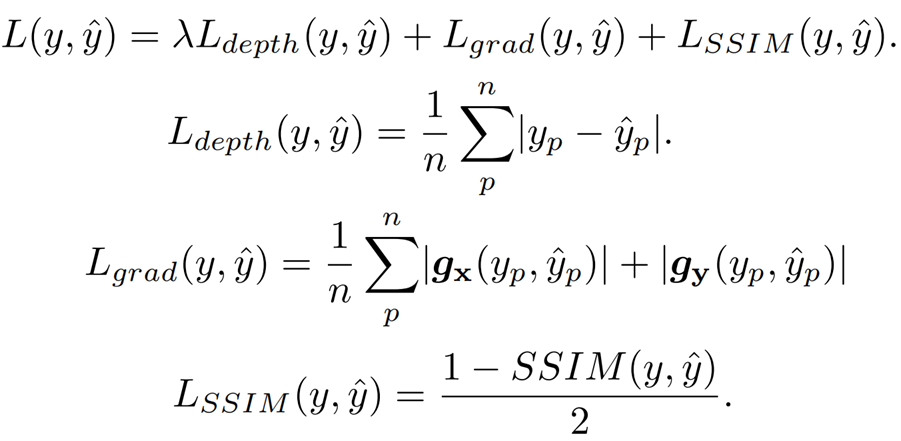
\includegraphics[width=.7\textwidth]{Images//unet6.png}
  \caption{تابع هزینه شبکه \lr{Unet}}\label{unet_loss}
\end{figure}

شبکه را با نرخ یادگیری آموزش $0.0001$، سایز بچ 4 و بهینه‌ساز آدام آموزش دادیم.
بعد از 10 مرحله آموزش حدود 84 درصد صحت روی داده‌های تست بدست آمد که درصد معقولی است.
در شکل \ref{unet_test} سه نمونه از تست‌های شبکه آورده شده‌است.
\begin{figure}
  \centering
  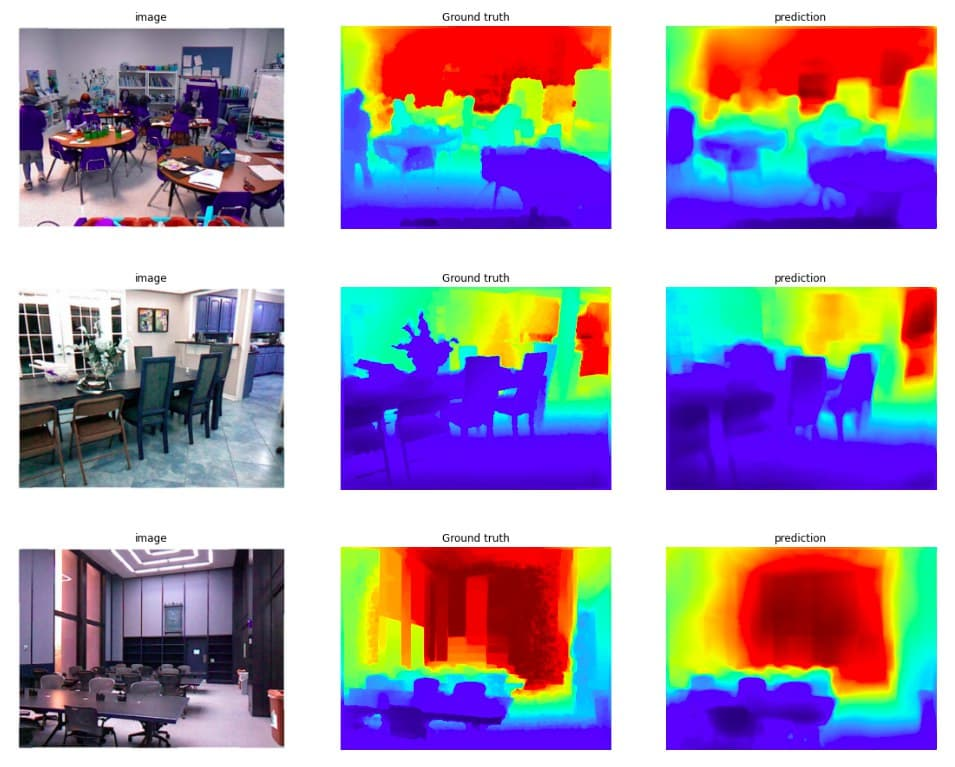
\includegraphics[width=\textwidth]{Images//unet_test.png}
  \caption{سه نمونه از تست های شبکه آموزش دیده}\label{unet_test}
\end{figure}

\chapter{آموزش مشترک}
در روش های مورد استفاده ما، شبکه‌های تشخیص اشیا و تشخیص عمق به صورت جداگانه از هم آموزش داده شده‌اند.
در خصوص اینکه آیا می توان شبکه ها را به صورت همزمان با هم آموزش داد و به دقت مطلوب رسید،
ما تحقیقاتی انجام دادیم.
در این رابطه ما با یک مسئله یادگیری چندوظیفه‌ای\LTRfootnote{Multi-Task Learning}
طرف هستیم.
جواب سوال احتمالا این است که می توانیم به همان دقت مطلوب یا حتی بیشتر برسیم.

در مورد یادگیری چندوظیفه‌ای مقالات مروری \cite{ruder2017overview} و \cite{zhang} را مطالعه کردیم.
طبق \cite{ruder2017overview} دو روش کلی برای آموزش مشترک شبکه‌های عصبی عمیق برای چند وظیفه وجود دارد.

اولی که اشتراک وزن سخت نام دارد، به این صورت است که تا تعدادی لایه، داده‌های موجود
در تمام وظایف از لایه های مشابه می‌گذرند و از جایی به بعد لایه‌های مخصوص وظایف وارد کار می‌شوند.
در حالت دوم که اشتراک وزن نرم نام دارد، هر وظیفه مدل خود را دارد، با وزن‌های و پارامترهای مخصوص خود.
در این روش قیدی رو وزن های مدل‌های مختلف گذاشته می‌شود تا وزن ها از هم فاصله زیادی نگیرند.
در شکل‌های \ref{joint_hard} و \ref{joint_soft} این حالت‌ها نمایش داده شده‌اند.
\begin{figure}[h]
  \centering
  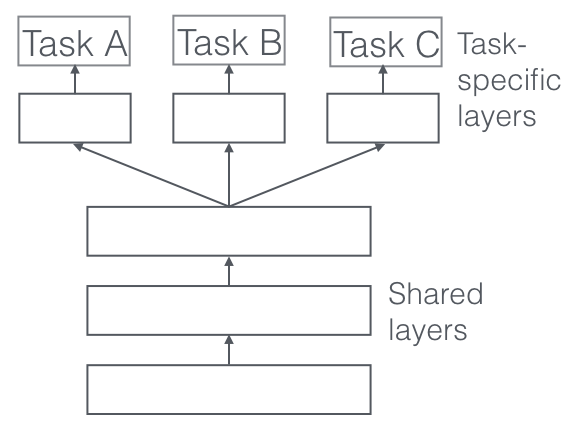
\includegraphics[width=.5\textwidth]{Images//joint1.png}
  \caption{اشتراک وزن سخت}\label{joint_hard}
\end{figure}
\begin{figure}[h]
  \centering
  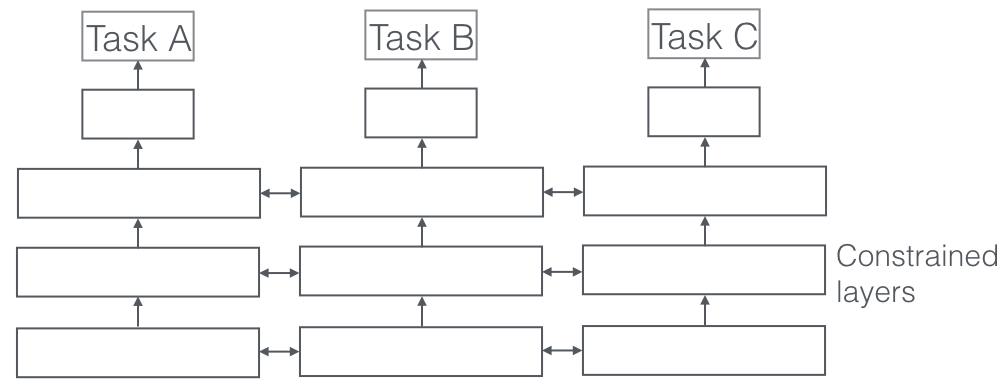
\includegraphics[width=.5\textwidth]{Images//joint2.png}
  \caption{اشتراک وزن نرم}\label{joint_soft}
\end{figure}

یادگیری چندوظیفه‌ای چند حسن دارد از جمله:
\begin{itemize}
  \item افزایش تعداد داده‌های آموزشی: در این روش‌ها به دلیل استفاده از داده‌های موجود در چند وظیفه مختلف، در صورت استفاده از یک ساختار مشترک تعداد داده‌های آموزشی ما خیلی بیشتر می شوند.
  \item تمرکز بیشتر روی ویژگی‌های اساسی: این مدل‌ها معمولا نسبتا نویز مقاومت خیلی بیشتری نشان می‌دهند.
  \item یادگیری ویژگی‌های راحت‌تر از دیگر وظابف: در این مدل‌ها معمولا ویژگی‌های مشترک بین وظایف به آموزش بهتر مدل کمک می‌کنند.
  \item رگولاریزاسیون: در این مسائل با اظافه شدن یک بایاس به مدل به دلیل وجود وظایف مختلف، احتمال
  بیش‌برازش و فیت شدن به نویز کمتر می‌شود.
\end{itemize}

در مطالعات ما، مقاله‌ای که از معیار ارزیابی مشترک برای مدل آموزش دیده استفاده کند یافت نشد.
روال کار همه مقالات به این صورت بود شبکه‌ها به صورت مشترک و جداگانه آموزش می‌دیدند،
و نهایتا با معیار ارزیابی هر وظیفه به صورت جداگانه ارزیابی می‌شدند.
با این تمام مقالات در حالت آموزش مشترک از یک \textbf{تابع هزینه مشترک} برای آموزش استفاده می‌کردند.
برای مثال در \cite{kendall2018multitask} از جمع وزن دار سه تابع هزینه جداگانه
برای وظایف \lr{sematic segmentation}، \lr{instance segmentation} و تشخیص عمق استفاده می‌شود.
برای وظیفه اول از آنتروپی متقابل پیکسل به پیکسل،
برای وظیفه دوم از نرم $L_1$
تفاضل \lr{instance} های یافت شده و برای وظیفه سوم از
نرم $L_1$ تفاضل پیکسل به پیکسل استفاده شده‌است.
در شکل \ref{joint_res} یک نمونه‌ای از نتایج این مقاله آورده شده‌است.
\begin{figure}
  \centering
  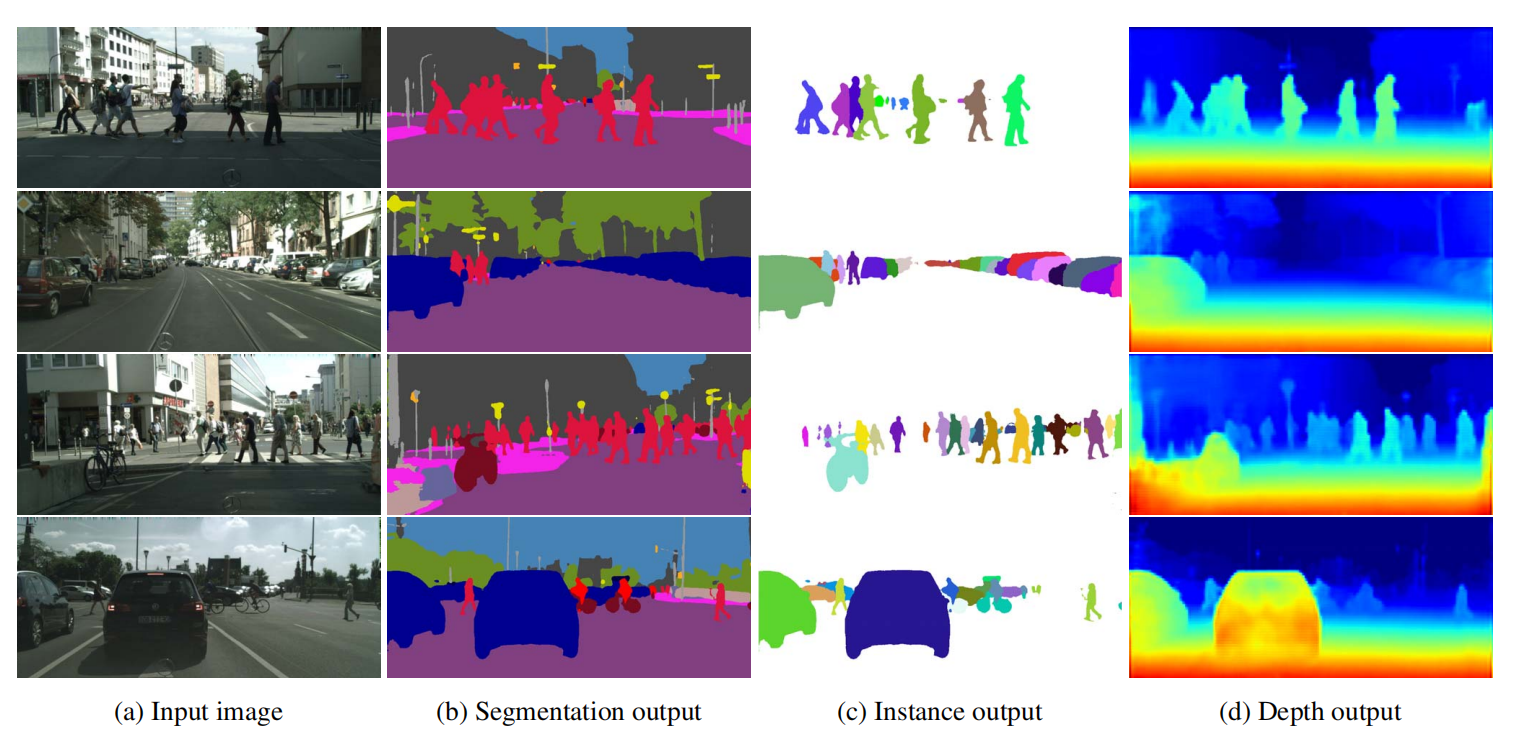
\includegraphics[width=\textwidth]{Images//joint3.png}
  \caption{مثالی از نتایج ساختار چندوظیفه ای مقاله \cite{kendall2018multitask}}\label{joint_res}
\end{figure}


\chapter{وب اپلیکیشن}
از دو روش برای ساختن وب اپلیکشن پروژه استفاده کردیم که در ادامه معرفی می‌شوند.
\section{\lr{Streamlit}}
برای اجرای این قسمت پس از دانلود وزن های مدل \lr{YOLO-v3} و نیز مدل و  وزن های  مدل آموزش داده شده \lr{Unet} و قرار دادن آن‌ها در پوشه‌های مورد نظر
(برای این کار تنها کافیست کدهای نوشته شده در \verb"README.md" را  به ترتیب اجرا کنید، این وزن‌ها به دلیل اینکه حجمشان بیشتر از ۱۰۰ مگابایت بود امکان آپلود در گیت‌هاب نداشتند.)
کد streamlit \verb"run ./src/app.py" را اجرا کنید تا برنامه روی لوکال هاست شما اجرا شود.
تعدادی از تصاویر داده شده به این وب اپلیکیشن را می‌توانید در شکل \ref{web_samp1} ببینید:

\begin{figure}
\centering
\subfloat{
  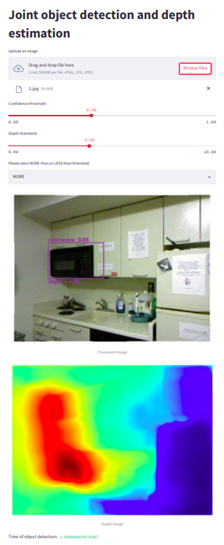
\includegraphics[width=0.3\textwidth]{Images//web1.png}
  \label{web1}}
\subfloat{
  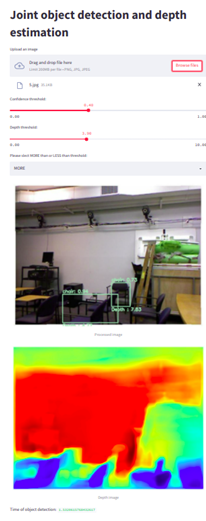
\includegraphics[width=0.3\textwidth]{Images//web2.png}
  \label{web2}}
  \centering
\subfloat{
  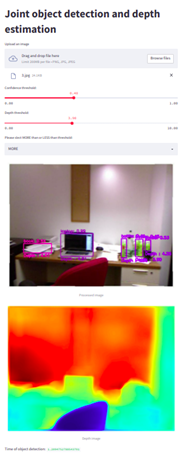
\includegraphics[width=0.3\textwidth]{Images//web3.png}
  \label{web3}}
\caption{نمونه های اجرای وب اپلیکیشن در حالت \lr{streamlit}}
\label{web_samp1}
\end{figure}

\section{\lr{Django}}
برای اجرای این قسمت پس از دانلود وزن‌های مدل \lr{YOLO-v3} و قرار دادن آن‌ها در پوشه مورد نظر (برای این کار تنها کافیست کدهای نوشته شده در \verb"README.md" را  به ترتیب اجرا کنید، این وزن‌ها به دلیل اینکه حجمشان بیشتر از ۱۰۰ مگابایت بود امکان آپلود در گیتهاب نداشتند.) کدهای ذکر شده در \verb"README.md" را اجرا کنید تا برنامه روی لوکال هاست شما اجرا شود.
تعدادی از تصاویر داده شده به این وب اپلیکیشن را میتوانید در شکل \ref{web_samp2} ببینید:
\begin{figure}
\centering
\subfloat{
  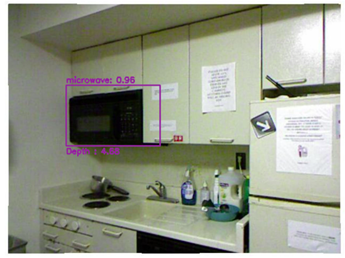
\includegraphics[width=0.35\textwidth]{Images//web4.png}
  \label{web4}}
\subfloat{
  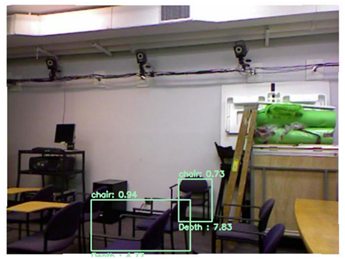
\includegraphics[width=0.35\textwidth]{Images//web5.png}
  \label{web5}}
  \centering
\subfloat{
  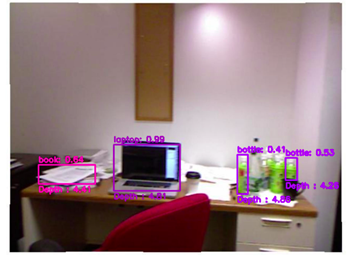
\includegraphics[width=0.35\textwidth]{Images//web6.png}
  \label{web6}}
\caption{نمونه های اجرای وب اپلیکیشن در حالت \lr{Django}}
\label{web_samp2}
\end{figure}

\section{چالش ها}
با توجه به این که باکس تشخیص داده شده توسط مدل تشخیص اشیاء لزوما شامل تصویر ما نیست (یک مستیطیل تماما انسان را تصور کنید!) برای اندازه‌گیری عمق، مستطیل داخلی باکس (هر ضلع سی درصد مستطیل تشخیص داده شده ی اصلی) را در نظر گرفتیم. برای پیشرفت کد و ادامه ی آن می‌توان مناطق مختلف تصویر را با توجه به کلاسی که تشخیص می‌دهیم در نظر گرفت یا خیر. برای مثال در تشخیص انسان با توجه به این که عمق انسان در تصویر تنها یک عدد است الگوریتم را تغییر نمیدهیم، اما در تشخیص میز با توجه به تغییر عمق آن میتوان یک عمق ابتدایی و انتهایی برای در نظر گرفت تا تشخیص آن دقیق‌تر باشد.

الگوریتم پیاده شده ما بر اساس مقاله ذکر شده در صورت پروژه است که مقدار را به روش زیر محاسبه کرده‌است:
\begin{figure}[h]
  \centering
  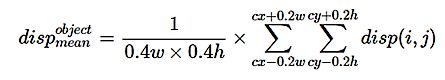
\includegraphics[width=.5\textwidth]{Images//web7.png}
  \label{web7}
\end{figure}

ریت مستطیل داخلی یک هایپرپارامتر است که ما هر ضلع را برابر سی درصد مسطیل تشخیص داده شده در نظر گرفتیم.
روش دیگر ارایه شده توسط مقاله به دست آوردن \lr{median} مقادیر بود:
\begin{figure}[h]
  \centering
  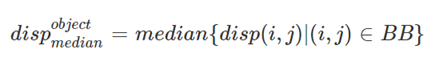
\includegraphics[width=.5\textwidth]{Images//web8.png}
  \label{web8}
\end{figure}

\newpage
\bibliographystyle{unsrt-fa}
\addtocontents{toc}{\textbf{مراجع}~\hfill\textbf{\thepage}\par}
{\small
\bibliography{References}}
\end{document} 